\documentclass[11pt,spanish]{article} % Tipo y tamaño de letra del documento.

\input{preamble.tex}

\newcommand{\tnum}{1} % reemplace 1 por el número de la tarea
\newcommand{\sem}{2026-1} % reemplace 2024-2 por el semestre correspondiente
\newcommand{\campus}{San Joaquin \\ Santiago} % reemplace Casa Central por el campus correspondiente
\newcommand{\rolusm}{202373514-0} % reemplace 2025073100-1 por su rol
\newcommand{\namestudent}{Vicente Silva Rios} % reemplace Al Goritmo Pérez por su nombre
\newcommand{\deadline}{9 de Abril de 2026} % reemplace POR DEFINIR por la fecha de entrega

\headheight=14pt
\linespread{1.3}
\author{\namestudent}
\pagestyle{fancy}
\fancyhf{}%
\fancyfoot[R]{ \namestudent \\ \rolusm}
\fancyfoot[L]{Campus \campus}
\fancyfoot[C]{\thepage}
\rhead{\sem}
\lhead{INF-221}
\renewcommand{\headrulewidth}{0.4pt}
\renewcommand{\footrulewidth}{0.4pt}
\newbool{programs}
\boolfalse{programs}
\chead{REPORTE TAREA \tnum~}



\title{
  \huge
  \textbf{REPORTE TAREA \tnum~ \\ ALGORITMOS Y COMPLEJIDAD} \\[1ex]
  \emph{\textquote{Más allá de la notación asintótica: Análisis experimental de algoritmos de ordenamiento y multiplicación de matrices.}}
  }


\date{
  \small
  \today\\
  \currenttime
}




\begin{document}
\maketitle
\thispagestyle{fancy}
\vspace{-1.0\baselineskip}

\section{Entorno experimental}
\begin{mdframed}
    \textbf{La extensión máxima para esta sección es de media página.}
\end{mdframed}

Especifique el hardware y software utilizado para realizar los experimentos (por ejemplo, procesador, memoria RAM, sistema operativo, compilador y versión). Incluya una mención breve de los datasets utilizados, los cuales son los descritos en el enunciado de la tarea.


\section{Resultados y Análisis}
\subsubsection{Multiplicación de matrices}

En la Figura se compara el tiempo de ejecución entre los algoritmos naive y Strassen para multiplicar matrices cuadradas hasta $N=256$, se saltaron las matrices con $N=1024$ debido a excesivo tiempo de ejecucion y hacer mas rapido la tarea, esto tambien en los algoritmos de ordenamiento, A medida que las matrices crecen, ambos aumentan su tiempo de acuerdo con sus complejidades teóricas. Aunque el algoritmo naive tiene una complejidad de $O(n^3)$, resulta más rápido en estas instancias evaluadas. Por su parte, Strassen reduce la complejidad a $O(n^{2.81})$, pero añade un costo extra debido a sus operaciones recursivas y al uso de memoria intermedia. Por lo tanto, para matrices pequeñas y medianas, la estrategia tradicional es más eficiente en la práctica.

Cabe destacar que estos datos se obtuvieron de forma automática. Los archivos \texttt{.csv} están disponibles en el repositorio del proyecto para que los resultados puedan ser verificados o reproducidos fácilmente.

\begin{figure}[H]
    \centering
    \begin{minipage}[t]{0.4\textwidth}
        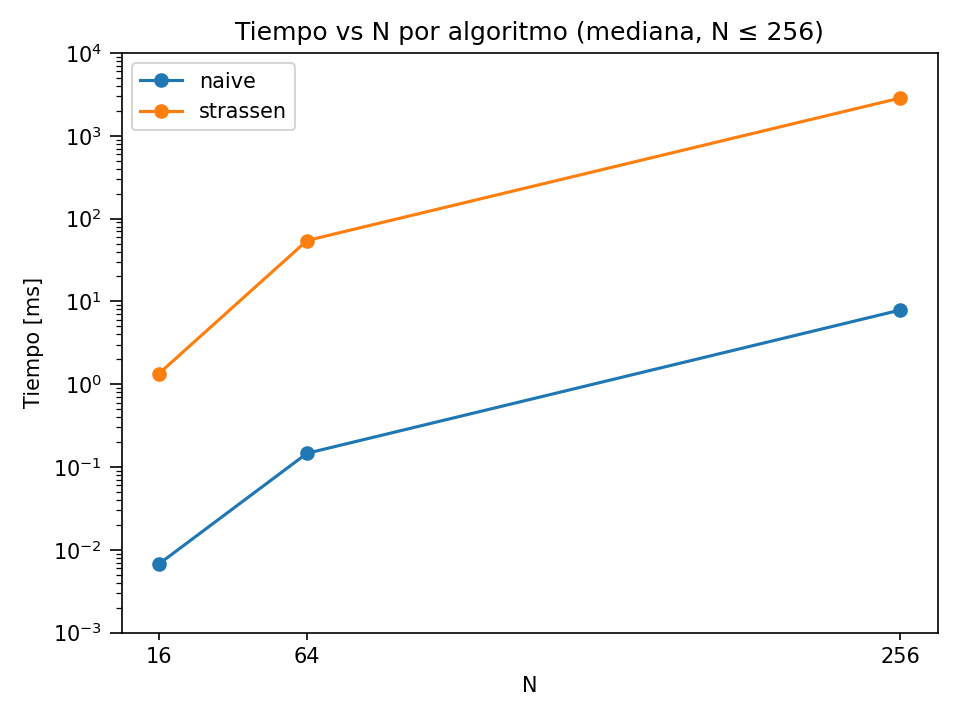
\includegraphics[width=\textwidth]{../code/matrix_multiplication/data/plots/t_vs_n_by_algo.png}
    \end{minipage}
    \caption{Gráfica de Tiempo vs N entre algoritmos.}
\end{figure}


\subsubsection{Efecto del tipo de matriz en el tiempo de ejecución}

Las Figuras muestran cómo varía el tiempo según el tipo de matriz (densa, diagonal o dispersa) y sus dominios D0 y D10.

\begin{figure}[H]
    \centering
    \begin{minipage}[t]{0.4\textwidth}
        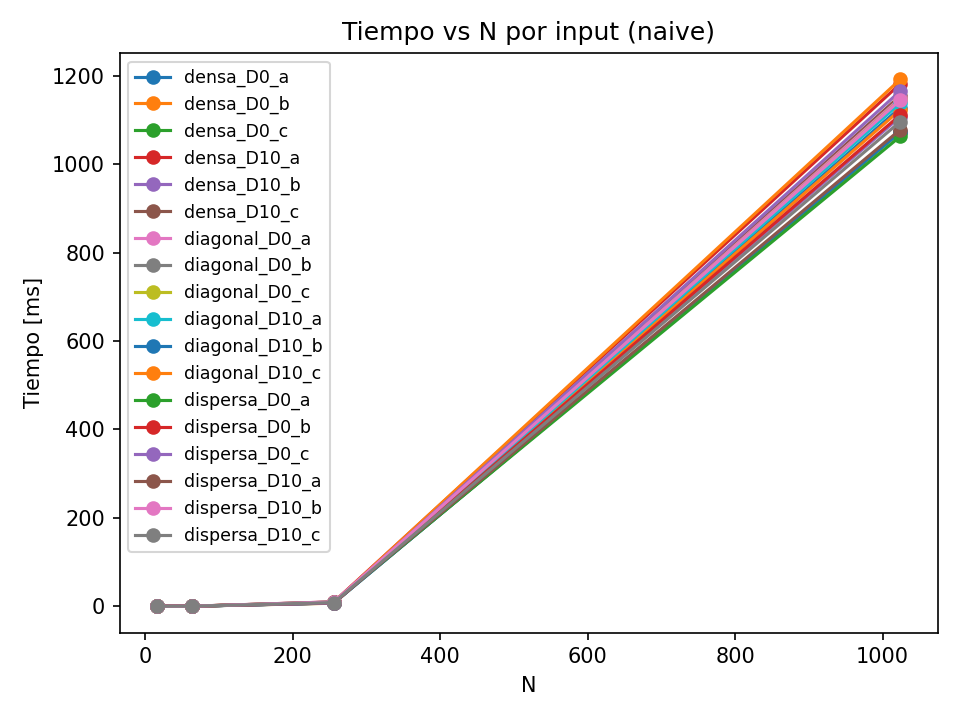
\includegraphics[width=\textwidth]{../code/matrix_multiplication/data/plots/t_vs_n_by_input_naive.png}
    \end{minipage}%
    \hspace{0.05\textwidth}
    \begin{minipage}[t]{0.4\textwidth}
        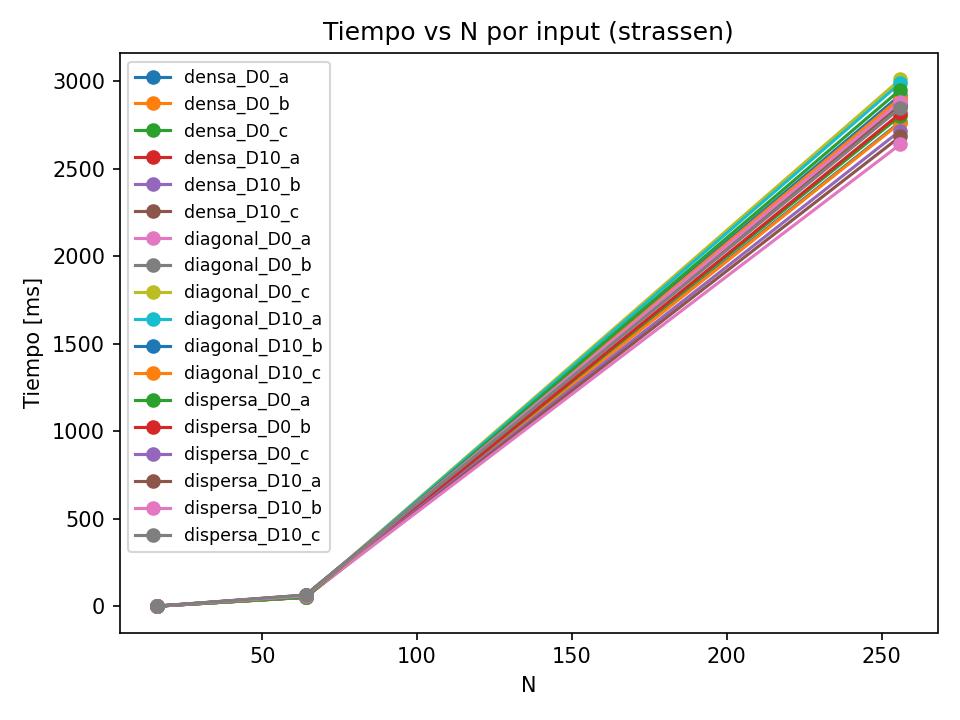
\includegraphics[width=\textwidth]{../code/matrix_multiplication/data/plots/t_vs_n_by_input_strassen.png}
     \end{minipage}
    \caption{Tiempo vs N por input de cada algoritmo.}
\end{figure}

El algoritmo naive tarda menos con matrices dispersas y luego con las diagonales, ya que evita realizar cálculos innecesarios con los ceros, reduciendo así la cantidad efectiva de multiplicaciones y sumas. En contraste, Strassen mantiene tiempos muy similares sin importar el tipo de matriz. Esto ocurre porque sus divisiones recursivas ejecutan secuencias fijas de operaciones que no logran aprovechar la presencia de ceros. En síntesis, naive saca ventaja de estructuras simples o vacías, mientras que Strassen es insensible a este factor.


\subsubsection{Memoria estimada en algoritmos de matrices}

La Figura ilustra la memoria estimada para instancias de hasta $256 \times 256$. Se observa que Strassen consume constantemente más memoria que el método naive, lo cual coincide con las estimaciones teóricas:
\[
M_{\text{naive}} \approx 3 \cdot n^2 \cdot \texttt{sizeof(int)}, \quad 
M_{\text{strassen}} \approx 8 \cdot n^2 \cdot \texttt{sizeof(int)}.
\]

\begin{figure}[H]
    \centering
    \begin{minipage}[t]{0.4\textwidth}
        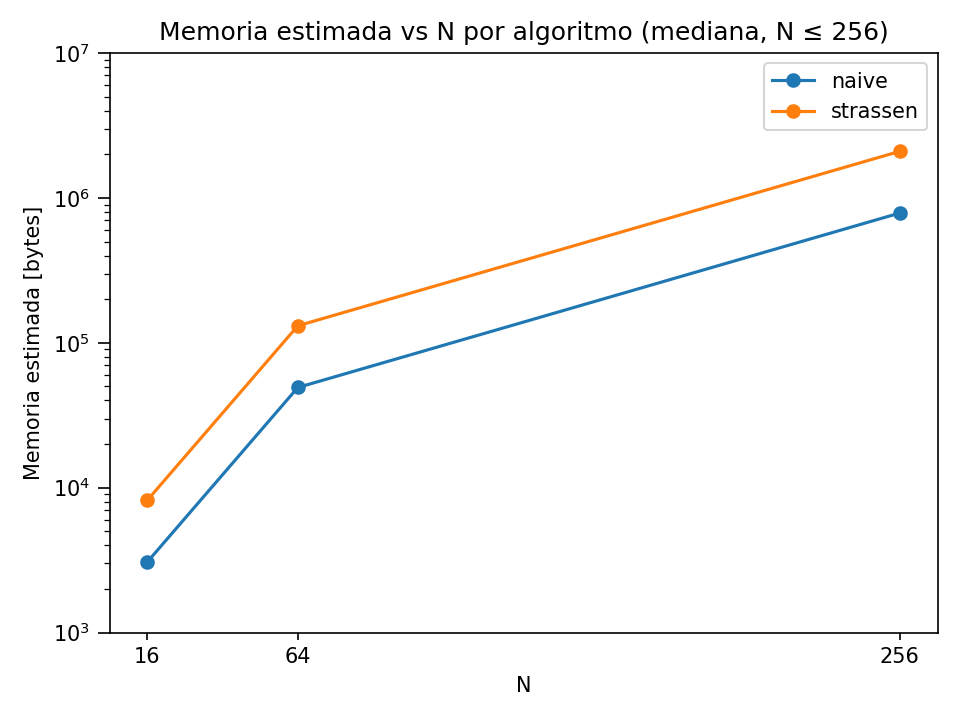
\includegraphics[width=\textwidth]{../code/matrix_multiplication/data/plots/mem_vs_n_by_algo.png}
    \end{minipage}
    \caption{Gráfica de Memoria estimada en función de N para los 2 algoritmos.}
\end{figure}

Esta diferencia radica en que naive opera directamente sobre las matrices originales y la resultante, mientras que Strassen exige generar múltiples submatrices en cada paso recursivo. Como conclusión, para tamaños moderados, Strassen resulta ser más lento y más demandante en memoria, limitando su atractivo frente a la versión tradicional.


\subsubsection{Algoritmos de ordenamiento de arreglos según el input}

En las 3 figuras se presentan los tiempos de ejecución de los algoritmos ( merge sort,  quick sort y std:sort) para distintos tamaños $n$ y tipos de entrada (ascendente, descendente y aleatorio). 

\begin{figure}[H]
    \centering
    \begin{minipage}[t]{0.32\textwidth}
        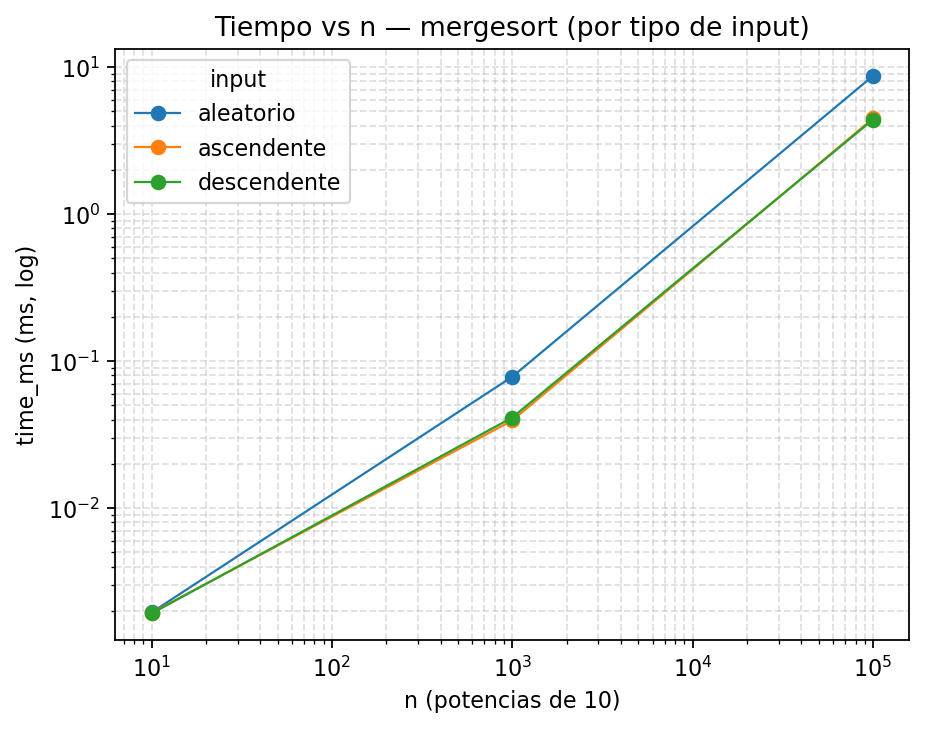
\includegraphics[width=\textwidth]{../code/sorting/data/plots/time_vs_n_mergesort.png}
    \end{minipage}\hfill
    \begin{minipage}[t]{0.32\textwidth}
        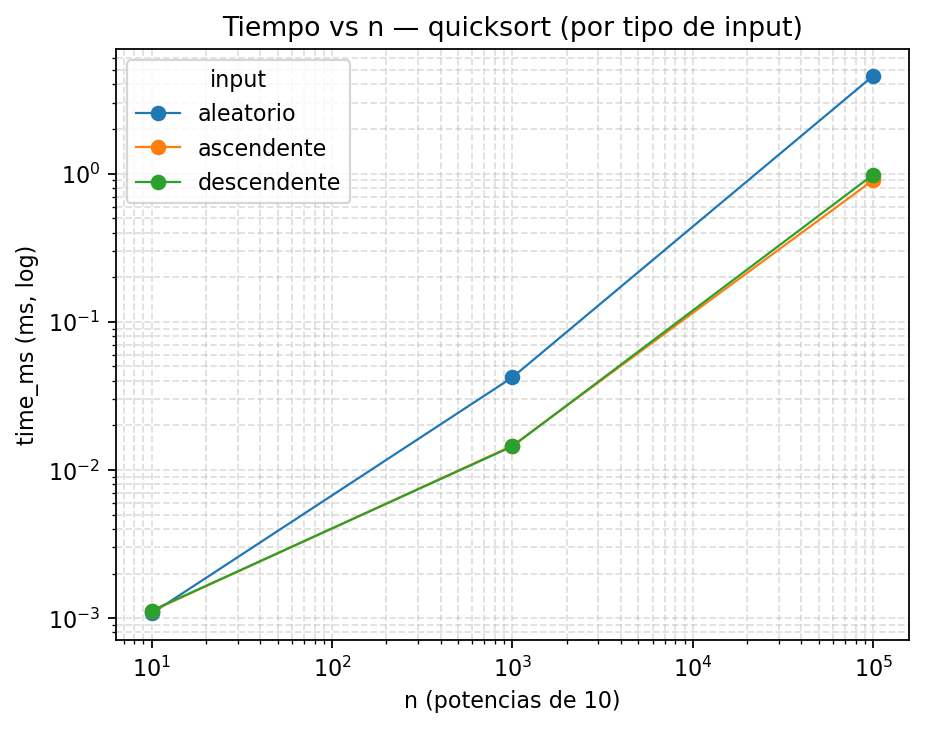
\includegraphics[width=\textwidth]{../code/sorting/data/plots/time_vs_n_quicksort.png}
    \end{minipage}\hfill
    \begin{minipage}[t]{0.32\textwidth}
        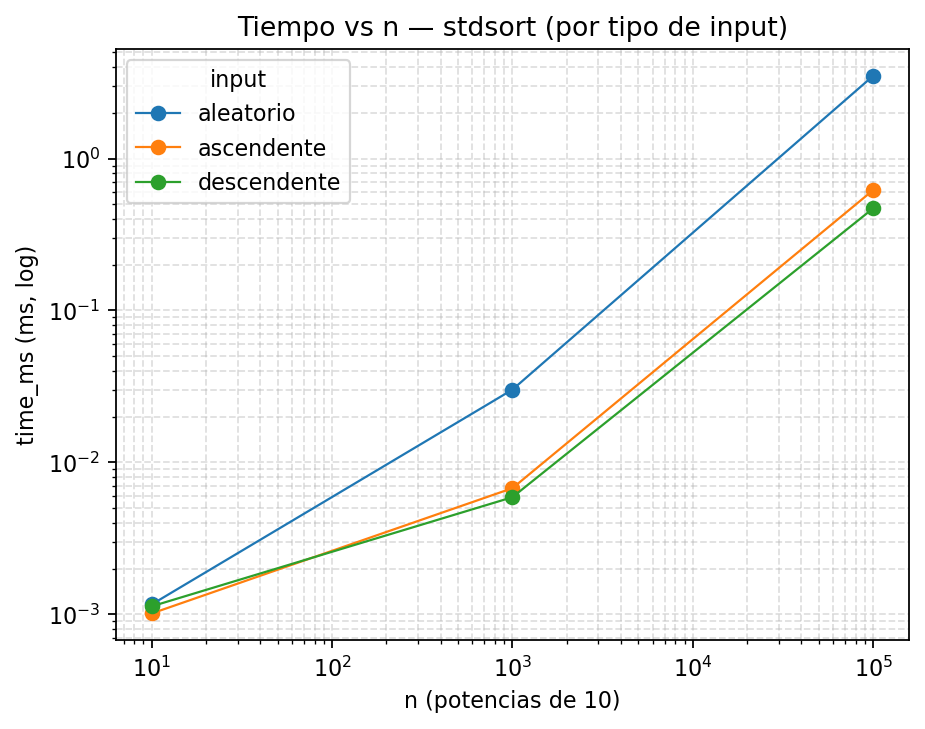
\includegraphics[width=\textwidth]{../code/sorting/data/plots/time_vs_n_stdsort.png}
    \end{minipage}
    \caption{Tiempo vs N por input de cada algoritmo.}
\end{figure}

Merge sort, fiel a su complejidad teórica de $O(n \log n)$, rinde igual en cualquier caso, mostrando solo un levísimo aumento de tiempo en los escenarios aleatorios. 

Quick sort, al utilizar un pivote central, es más lento en arreglos aleatorios debido a que los arreglos ya ordenados le generan particiones mucho más balanceadas. En resumen, los algoritmos cuadráticos dependen fuertemente del orden original de los datos, mientras que los más eficientes mantienen un rendimiento estable.

std::sort, fiel a su complejidad teórica de $O(n \log n)$, garantiza eficiencia en todos los escenarios, pero muestra un tiempo de ejecución notablemente mayor frente a los arreglos aleatorios, al estar altamente optimizado para detectar y aprovechar secuencias existentes, procesa los arreglos preordenados en tiempos casi idénticos y mucho más rápidos al minimizar drásticamente los intercambios en memoria.

\subsubsection{Memoria estimada en algoritmos de ordenamiento}

En la Figura se expone el uso máximo de memoria extra en función del tamaño del arreglo $n$ para los algoritmos evaluados.

\begin{figure}[H]
    \centering
    \begin{minipage}[t]{0.45\textwidth}
        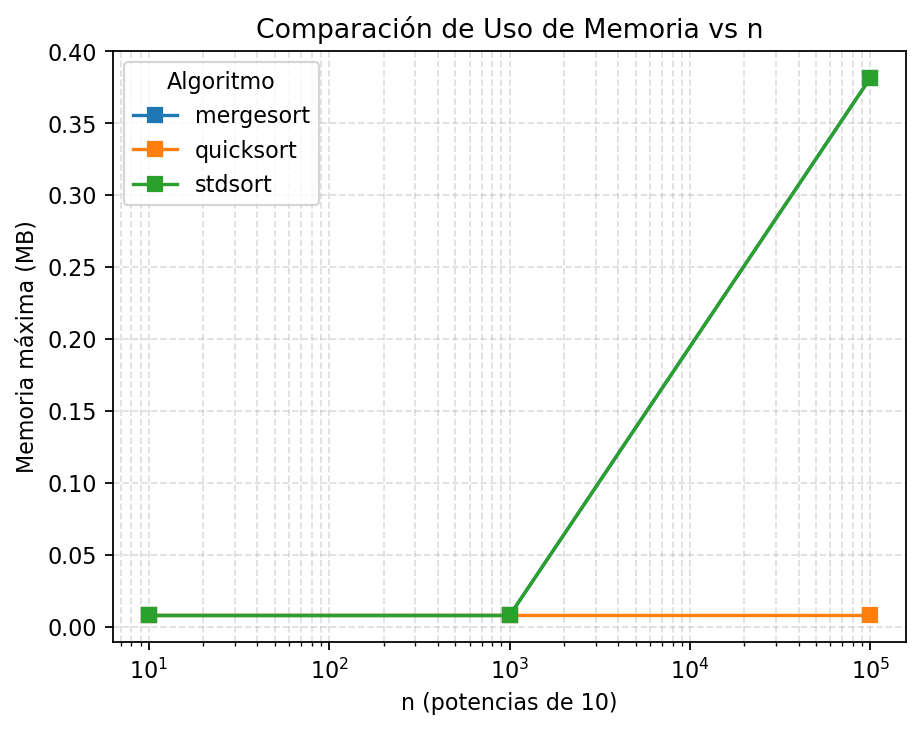
\includegraphics[width=\textwidth]{../code/sorting/data/plots/memory_comparison_vs_n.png}
    \end{minipage}
    \caption{Comparación de uso de memoria vs n entre algoritmos de ordenamiento.}
\end{figure}

Se evidencia que quicksort mantiene un consumo de memoria extra prácticamente nulo en todos los casos, lo que confirma experimentalmente su naturaleza de ordenamiento.

Por el contrario, tanto mergesort como stdsort muestran un crecimiento lineal que se superpone perfectamente en el gráfico, alcanzando exactamente 400,000 bytes para los arreglos de $10^5$ elementos.

En el caso de mergesort, este aumento concuerda con su complejidad espacial teórica de $O(n)$, ya que el algoritmo requiere instanciar arreglos temporales para poder fusionar las mitades.

\section{Conclusiones}
\begin{mdframed}
    \textbf{La extensión máxima para esta sección es un párrafo breve (máximo 1/4 de página).}
\end{mdframed}

Escriba una conclusión breve que interprete los resultados más importantes. Cada afirmación debe estar respaldada por los datos presentados.


\printbibliography

\end{document}
